
\documentclass[conference]{IEEEtran}

% =========================
% Packages
% =========================
\usepackage{cite}
\usepackage{amsmath,amssymb,amsfonts}
\usepackage{algorithm}
\usepackage{algpseudocode}
\usepackage{graphicx}
\usepackage{textcomp}
\usepackage{xcolor}
\usepackage{booktabs}
\usepackage{multirow}
\usepackage{url}
\usepackage{tikz}
\usetikzlibrary{arrows.meta, positioning, shapes.geometric}

\begin{document}

% =========================
% Title and Authors
% =========================
\title{TrailGuard TW: An Evidence-Based Mountain Risk Decision Support Agent for Taiwan}

\author{
\IEEEauthorblockN{Author Name}
\IEEEauthorblockA{
Department of Computer Science\\
University Name\\
Taiwan\\
Email: author@example.com
}
}

\maketitle

% =========================
% Abstract
% =========================
\begin{abstract}
Mountain safety has become an increasingly important issue in Taiwan.
Following the promotion of the Open Mountain initiative in 2019,
mountain access has become more convenient; however, hikers continue
to face risks caused by fragmented information, rapidly changing
weather conditions, and inadequate pre-trip decision-making.

Existing mountain information services typically provide weather
forecasts, route descriptions, and safety announcements separately.
Hikers must manually integrate these heterogeneous sources to assess
route feasibility and potential risks. This process is time-consuming
and may lead to incomplete or outdated decisions.

This paper proposes TrailGuard TW, an evidence-based mountain risk
decision support agent that integrates large language models (LLMs),
a deterministic Python risk assessment engine, and a temporal
knowledge graph. The proposed system evaluates hiking feasibility
using estimated travel time, weather windows, altitude-related risks,
and time-sensitive safety information. An Evidence Ledger is
introduced to maintain traceability between recommendations and
their supporting sources. Furthermore, critical safety conditions
are implemented as hard constraints to prevent an LLM from overriding
high-risk warnings.

A simulation-based evaluation framework is designed to assess
decision reliability, evidence traceability, and risk identification
performance. The proposed approach aims to improve the transparency,
consistency, and reliability of pre-trip mountain safety decisions.
\end{abstract}

\begin{IEEEkeywords}
Mountain Safety, Large Language Models, Decision Support System,
Temporal Knowledge Graph, Risk Assessment, Evidence-Based AI
\end{IEEEkeywords}

% =========================
% I. Introduction
% =========================
\section{Introduction}

Taiwan has abundant high-mountain resources and diverse hiking
environments. With the promotion of the Open Mountain initiative
in 2019, public access to mountain activities has become more
convenient. However, mountain accidents remain an important
challenge for outdoor safety management.

According to the statistics collected for this study, getting lost
accounts for 38.61\% of mountain accidents, while self-organized
groups account for 55.85\%. These figures suggest that inadequate
pre-trip planning and insufficient risk awareness may contribute
to mountain incidents.

Before a hiking activity, hikers generally need to collect
information from multiple sources, including weather forecasts,
trail conditions, route descriptions, altitude information,
and official safety announcements. Since these sources are
distributed across different platforms and may have different
update frequencies, hikers must manually determine whether the
information is consistent and still valid.

Large language models provide a convenient interface for
natural-language interaction and information summarization.
However, an LLM may generate unsupported statements or fail to
recognize critical safety constraints. Therefore, relying solely
on generative AI for mountain safety decisions is insufficient.

To address these challenges, this paper proposes TrailGuard TW,
an evidence-based mountain risk decision support agent.

The main contributions are summarized as follows:

\begin{itemize}
    \item We propose an integrated architecture combining an LLM,
    a deterministic Python risk engine, and a temporal knowledge
    graph for mountain risk assessment.

    \item We introduce an Evidence Ledger to associate each
    recommendation with its source, timestamp, and validity period.

    \item We design hard safety constraints that prevent the
    system from recommending a route when critical risk conditions
    are detected.

    \item We establish a simulation-based evaluation framework
    for measuring decision reliability, evidence traceability,
    and risk identification performance.
\end{itemize}

% =========================
% II. Related Work
% =========================
\section{Related Work}

\subsection{Mountain Safety Information Systems}

Traditional mountain safety systems provide information such as
weather forecasts, route descriptions, and emergency announcements.
However, these services are often distributed across different
websites and platforms.

The lack of integration increases the cognitive burden on hikers
and makes it difficult to evaluate the combined impact of multiple
risk factors.

\subsection{Large Language Models for Decision Support}

Large language models have demonstrated strong capabilities in
natural-language understanding, question answering, and information
summarization.

Nevertheless, LLM-generated responses may contain hallucinated
information or unsupported conclusions. In safety-critical
applications, generated recommendations should therefore be
verified against reliable external evidence.

\subsection{Knowledge Graphs and Temporal Information}

Knowledge graphs represent entities and their relationships in a
structured format. Temporal knowledge graphs further associate
information with time-related attributes, allowing systems to
reason about the validity of changing information.

In mountain safety applications, temporal information is important
because weather forecasts, trail closures, and safety announcements
may become outdated.

% =========================
% III. Proposed Framework
% =========================
\section{Proposed Framework}

\subsection{System Architecture}

TrailGuard TW consists of four major components:

\begin{enumerate}
    \item \textbf{LLM Interface:} Understands user queries and
    generates natural-language explanations.

    \item \textbf{Python Risk Engine:} Performs deterministic
    calculations for travel time, weather windows, and risk scores.

    \item \textbf{Temporal Knowledge Graph:} Stores mountain
    routes, weather conditions, safety announcements, and
    their temporal validity.

    \item \textbf{Evidence Ledger:} Records the sources and
    timestamps supporting each recommendation.
\end{enumerate}

\begin{figure}[!t]
\centering
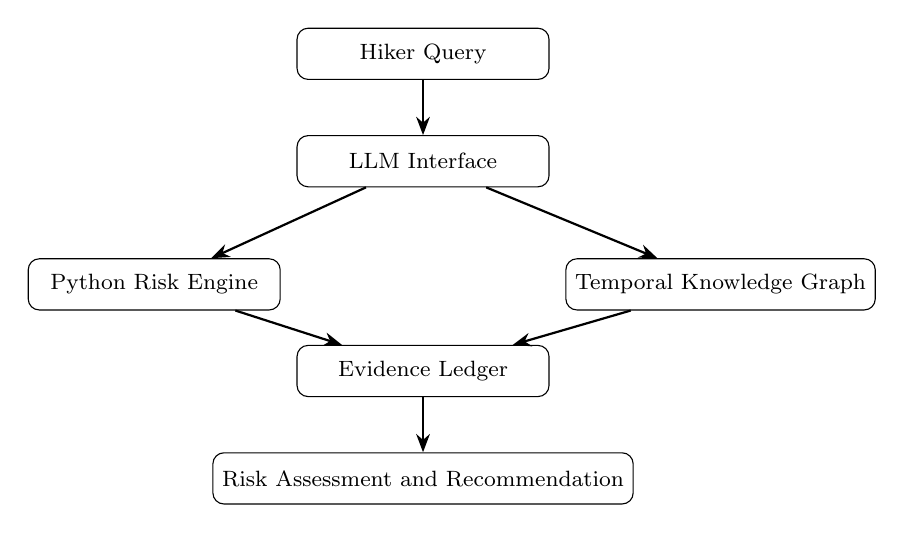
\begin{tikzpicture}[
    node distance=0.7cm,
    block/.style={
        rectangle,
        draw,
        rounded corners,
        align=center,
        minimum width=3.2cm,
        minimum height=0.65cm,
        font=\footnotesize
    },
    arrow/.style={-{Stealth}, thick}
]

\node[block] (user) {Hiker Query};

\node[block, below=of user] (llm) {LLM Interface};

\node[block, below left=0.9cm and 0.2cm of llm]
    (engine) {Python Risk Engine};

\node[block, below right=0.9cm and 0.2cm of llm]
    (graph) {Temporal Knowledge Graph};

\node[block, below=1.0cm of llm, yshift=-1.0cm]
    (ledger) {Evidence Ledger};

\node[block, below=of ledger] (output)
    {Risk Assessment and Recommendation};

\draw[arrow] (user) -- (llm);
\draw[arrow] (llm) -- (engine);
\draw[arrow] (llm) -- (graph);
\draw[arrow] (engine) -- (ledger);
\draw[arrow] (graph) -- (ledger);
\draw[arrow] (ledger) -- (output);

\end{tikzpicture}
\caption{Overall architecture of TrailGuard TW.}
\label{fig:architecture}
\end{figure}

\subsection{Travel Time Estimation}

The system estimates hiking duration using route distance,
elevation gain, and terrain-related factors.

A simplified travel-time model can be expressed as:

\begin{equation}
T_{\mathrm{total}} =
T_{\mathrm{ascent}} +
T_{\mathrm{descent}} +
T_{\mathrm{rest}}
\label{eq:travel}
\end{equation}

To represent uncertainty, the system considers both the median
and the 90th-percentile travel-time estimates:

\begin{equation}
T_{\mathrm{P50}} = Q_{0.50}(T)
\end{equation}

\begin{equation}
T_{\mathrm{P90}} = Q_{0.90}(T)
\end{equation}

where $Q_p(T)$ represents the $p$-th percentile of estimated
travel time.

\subsection{Temporal Validity Assessment}

Information from external sources may become outdated.
Each evidence item is associated with a timestamp and a validity
period.

The validity of evidence item $e_i$ at time $t$ is defined as:

\begin{equation}
V(e_i,t) =
\begin{cases}
1, & t \leq t_i + \Delta_i \\
0, & \text{otherwise}
\end{cases}
\label{eq:validity}
\end{equation}

where $t_i$ is the collection time and $\Delta_i$ is the
validity duration.

\subsection{Hard Safety Constraints}

To prevent unsafe recommendations, TrailGuard TW introduces
hard safety constraints.

Let $R$ represent the set of critical risk conditions.
The final recommendation is defined as:

\begin{equation}
Decision =
\begin{cases}
NO\text{-}GO, & \exists r_i \in R,\ r_i=1 \\
GO, & \text{otherwise}
\end{cases}
\label{eq:decision}
\end{equation}

Critical conditions may include official trail closures,
severe weather warnings, or other predefined safety restrictions.

The LLM is responsible for explaining the decision, while the
deterministic risk engine enforces the safety constraints.

\subsection{Evidence Ledger}

The Evidence Ledger records the supporting information for
each recommendation.

Each evidence record contains:

\begin{itemize}
    \item Evidence identifier
    \item Source name and URL
    \item Collection timestamp
    \item Validity period
    \item Related risk factor
    \item Decision contribution
\end{itemize}

The design follows a fundamental principle:

\begin{quote}
No source, no number.
\end{quote}

In other words, numerical claims and safety recommendations
should be traceable to supporting evidence.

\subsection{Decision Algorithm}

Algorithm~\ref{alg:trailguard} illustrates the proposed
decision-making procedure.

\begin{algorithm}[!t]
\caption{TrailGuard TW Risk Assessment}
\label{alg:trailguard}
\begin{algorithmic}[1]
\Require User query, route data, weather data, safety notices
\Ensure Risk assessment and recommendation

\State Parse user query using LLM
\State Retrieve relevant route information
\State Retrieve weather and safety information
\State Validate evidence timestamps

\State Estimate $T_{\mathrm{P50}}$ and $T_{\mathrm{P90}}$
\State Calculate risk indicators

\If{critical safety condition is detected}
    \State decision $\gets$ NO-GO
\Else
    \State decision $\gets$ GO
\EndIf

\State Generate evidence-backed explanation
\State Store evidence in Evidence Ledger

\Return decision and explanation
\end{algorithmic}
\end{algorithm}

% =========================
% IV. Experimental Design
% =========================
\section{Experimental Design}

\subsection{Simulation Scenarios}

A simulation dataset containing 120 mountain hiking scenarios
is planned for evaluating the proposed system.

The scenarios will cover different combinations of:

\begin{itemize}
    \item Weather conditions
    \item Route difficulty
    \item Hiking duration
    \item Elevation gain
    \item Official safety warnings
    \item Information freshness
\end{itemize}

Each scenario will be labeled according to its expected
risk category and recommended decision.

\subsection{Baseline Methods}

The proposed approach will be compared with the following methods:

\begin{itemize}
    \item \textbf{LLM-only:} Uses an LLM to generate recommendations
    without deterministic risk verification.

    \item \textbf{Rule-based:} Uses predefined rules to evaluate
    route feasibility.

    \item \textbf{RAG-based:} Retrieves external information and
    generates recommendations using an LLM.

    \item \textbf{TrailGuard TW:} Integrates LLM reasoning,
    deterministic risk assessment, temporal information,
    and evidence tracking.
\end{itemize}

\subsection{Evaluation Metrics}

The evaluation focuses on decision safety and evidence quality.

\subsubsection{False-Safe Rate}

False-Safe Rate (FSR) measures the proportion of unsafe scenarios
incorrectly classified as safe:

\begin{equation}
FSR =
\frac{N_{\mathrm{unsafe\rightarrow safe}}}
{N_{\mathrm{unsafe}}}
\label{eq:fsr}
\end{equation}

A lower FSR indicates better safety performance.

\subsubsection{Citation Success Rate}

Citation Success Rate (CSR) measures the proportion of claims
supported by valid evidence:

\begin{equation}
CSR =
\frac{N_{\mathrm{supported\ claims}}}
{N_{\mathrm{total\ claims}}}
\label{eq:csr}
\end{equation}

\subsubsection{Mean Absolute Percentage Error}

Travel-time estimation accuracy is evaluated using MAPE:

\begin{equation}
MAPE =
\frac{100\%}{n}
\sum_{i=1}^{n}
\left|
\frac{y_i-\hat{y}_i}{y_i}
\right|
\label{eq:mape}
\end{equation}

where $y_i$ is the actual travel time and $\hat{y}_i$
is the estimated travel time.

\subsection{Ablation Study}

An ablation study will be conducted to investigate the
contribution of individual components.

The following configurations are considered:

\begin{itemize}
    \item Without the deterministic Python risk engine
    \item Without temporal validity checking
    \item Without the Evidence Ledger
    \item Without hard safety constraints
\end{itemize}

The results will help identify which components contribute
most significantly to system reliability.

% =========================
% V. Results and Discussion
% =========================
\section{Results and Discussion}

This section will present the experimental results after
the simulation and evaluation have been completed.

The comparison will focus on:

\begin{enumerate}
    \item False-Safe Rate across different methods.
    \item Evidence traceability and citation validity.
    \item Travel-time estimation accuracy.
    \item System performance under outdated or conflicting
    information.
    \item The effectiveness of hard safety constraints.
\end{enumerate}

\begin{table}[!t]
\centering
\caption{Experimental Results Comparison}
\label{tab:results}
\begin{tabular}{lccc}
\toprule
Method & FSR & CSR & MAPE \\
\midrule
LLM-only & TBD & TBD & TBD \\
Rule-based & TBD & TBD & TBD \\
RAG-based & TBD & TBD & TBD \\
TrailGuard TW & TBD & TBD & TBD \\
\bottomrule
\end{tabular}
\end{table}

The values in Table~\ref{tab:results} should be replaced with
actual experimental measurements. No experimental performance
is assumed in this template.

% =========================
% VI. Conclusion
% =========================
\section{Conclusion}

This paper proposes TrailGuard TW, an evidence-based mountain
risk decision support agent designed to improve pre-trip
mountain safety decisions in Taiwan.

The proposed architecture integrates large language models,
a deterministic Python risk engine, a temporal knowledge graph,
and an Evidence Ledger. By separating natural-language
interaction from deterministic safety verification, the system
aims to reduce unsupported recommendations and improve
decision traceability.

Furthermore, hard safety constraints provide an additional
safeguard against critical risks, while temporal validity
checking helps prevent outdated information from influencing
recommendations.

Future work will focus on implementing the complete system,
collecting real-world mountain scenarios, and conducting
comprehensive experiments to evaluate its reliability and
practical effectiveness.

% =========================
% Acknowledgment
% =========================
\section*{Acknowledgment}

The authors would like to thank the relevant organizations
and data providers for their publicly available mountain,
weather, and safety information.

% =========================
% References
% =========================
\bibliographystyle{IEEEtran}
\bibliography{references}

\end{document}
